Being able to type up your mathematical writing is a beneficial skill to have, and is one that is expected of anyone working in a mathematical field. Unfortunately, most Office-style {\small WYSIWYG} (`what you see is what you get') text editors are not designed for this task---it becomes quickly cumbersome to deal with complicated mathematical notation, and fast alternations between notation and prose.

\LaTeX{} is a markup language that allows you to input both text and mathematical notation, inputting all mathematical notation, text formatting and document structure as code. What follows is a brisk introduction to \LaTeX{}, that should suffice for the purposes of this book.

The word \LaTeX{} is pronounced like `\textsc{lay}-tek' or `\textsc{lah}-tek', with a hard `k' sound---the `X' is meant to resemble the Greek letter \textit{chi} ($\chi$), so is pronounced by some people as such. It doesn't really matter how you say it, but do be warned that if you pronounce it like `\textsc{lay}-teks' then people will think you're talking about something somewhat different.

\subsection*{Finding the software}

You can use \LaTeX{} by installing it on your computer, or by using a web-based editor. There are advantages and disadvantages to both.

\begin{itemize}
\item On a web-based editor, everything is set up and ready to go, but you have less control over how everything compiles and you need an internet connection at all times when editing your files.
\item On a computer, you have more control over how your files compile, you have access to all the logs and auxiliary files (I won't go into this) and you don't need an internet connection---but it can be harder to use different packages, you're at the mercy of your own machine's limitations, and it's more technically involved.
\end{itemize}

There are many online and computer-based options available, and the reader is encouraged to research their options, but as a starting point, I present here the \LaTeX{} implementations used for writing this book.

Much of the book was originally written using the online editor \textit{ShareLaTeX}, which has merged with \textit{Overleaf} as of September 2018 and can be accessed at the following URL:

\vspace{-15pt}
\begin{center}
\url{https://www.overleaf.com/}
\end{center}

\vspace{-15pt}
Installing \LaTeX{} on a computer is slightly more complicated. In order to make \LaTeX{} documents on your computer, you need both a \textit{compiler}, for turning the code into a readable document, and an \textit{editor}, for writing the code and facilitating the compilation process.

The compiler used for this book is \textit{TeX Live}:

\vspace{-15pt}
\begin{center}
\url{https://www.tug.org/texlive/}
\end{center}

\vspace{-15pt}
and the editor is \textit{TeXstudio}:

\vspace{-15pt}
\begin{center}
\url{https://www.texstudio.org/}
\end{center}

\vspace{-15pt}
Both TeX Live and TeXstudio are free, cross-platform and open-source.

\subsection*{Getting started}

When you have settled on an online \LaTeX{} editor or installed \LaTeX{} on your computer, you can start editing. The files containing the \LaTeX{} code are plain-text files with the file extension \texttt{.tex} and consists of two components: a \textit{header} and a \textit{body}. Worrying about the details of what goes in the header and what goes in the body is not recommended if you are new to \LaTeX{} so, with this in mind, a template can be downloaded from the book's website:

\vspace{-15pt}
\begin{center}
\url{\bookurl/latex/}
\end{center}

\vspace{-15pt}
The code is replicated at the end of this section, on page \pageref{pTeXTemplate}.

\newpage
\subsection*{Text mode and math mode}
Before we get into the nitty-gritty, I should mention the difference between `text mode' and `math mode'.

\begin{itemize}
\item \textbf{Text mode} is the default mode: the stuff you type will appear as text, and this is the mode you should use when writing anything that isn't mathematical notation.
\item You should use \textbf{math mode} when you're typing anything which is mathematical notation, including variables, numbers, fractions, square roots, powers, sums, products, binomial coefficients, and so on.
\end{itemize}

To enter math mode, enclose whatever mathematical notation you are writing with dollar signs (\texttt{\${}}). For example, if I type \lstinline|$E=mc^{2}$| then \LaTeX{} shows $E=mc^2$. Sometimes it is convenient to put longer expressions on their own line, in which case you can enclose it between \lstinline|\[| and \lstinline|\]|; for example, if I type
\begin{center}\lstinline|\[ a^{2}+b^{2}+c^{2}=ab+bc+ca \]|\end{center}
then \LaTeX{} displays \[ a^{2}+b^{2}+c^{2}=ab+bc+ca \] on a line all of its own.

If you need to type text inside math mode (enclosed by \texttt{\$} signs), you can do that using \lstinline|\text{...}|, for example:

\begin{texcodeleft}[1]
\[ \sum_{i=1}^n i = \frac{n(n+1)}{2} \text{ for all } n \in \mathbb{N} \]
\end{texcodeleft}

\begin{texcoderight}[1]
\[ \sum_{i=1}^n i = \frac{n(n+1)}{2} \text{ for all } n \in \mathbb{N} \]
\end{texcoderight}

Note the spaces before and after `for all'; had I left those out of the code, they would not appear because \LaTeX{} ignores spacing in math mode. You can force a space by putting a backslash before a space, for example \lstinline|$a b$| gives $a b$ but \lstinline|$a\ b$| gives $a\ b$.

\textbf{All} mathematical notation should be in math mode, including single variables. Notice the difference between the following two lines:
\[ \text{If a and b are both even then so is a+b.} \]
\[ \text{If } a \text{ and } b \text{ are both even then so is } a+b \text{.} \]
While the first is written entirely in text mode, the second is written using math mode for the variables and $+$ sign. Although the differences may not seem big, spread over a whole document it is much clearer when math mode is used (as in the second example). Sometimes ambiguities appear, and in any case \LaTeX{} does a much better job at displaying mathematical notation when it is typed in math mode.

\newpage
\subsection*{Table of mathematical symbols}

The following table is a quick reference for the most commonly-used symbols in this book. A complete index of notation can be found at the end of the book.

\begin{center}
\fitwidthc{0.95}{\begin{tabular}{|c|c|l|}

\hline \multicolumn{3}{|c|}{\textbf{Logic}} \\ \hline
conjunction, disjunction & $\wedge$, $\vee$ & \texcodebs{wedge}, \texcodebs{vee} \\
negation & $\neg$ & \texcodebs{neg} \\
implication, biconditional & $\Rightarrow$, $\Leftrightarrow$ & \texcodebs{Rightarrow}, \texcodebs{Leftrightarrow} \\
exclusive disjunction & $\oplus$ & \texcodebs{oplus} \\
true, false (in truth table) & $\checkmark$, $\times$ & \texcodebs{checkmark}, \texcodebs{times} \\
quantifiers (universal, existential) & $\forall$, $\exists$ & \texcodebs{forall}, \texcodebs{exists} \\

\hline \multicolumn{3}{|c|}{\textbf{Set theory}} \\ \hline
element, subset & $\in$, $\subseteq$ & \texcodebs{in}, \texcodebs{subseteq} \\
not equal, proper subset & $\ne$, $\subsetneqq$ & \texcodebs{ne}, \texcodebs{subsetneqq} \\
intersection, (indexed) & $\cap$, $\bigcap_{i=1}^{n}$ & \texcodebs{cap}, \texcodebs{bigcap\_\{i=1\}\^{}\{n\}} \\
union, (indexed) & $\cup$, $\bigcup_{i=1}^{n}$ & \texcodebs{cup}, \texcodebs{bigcup\_\{i=1\}\^{}\{n\}}  \\
relative complement, complement & $X \setminus Y$, $X^c$ & \texcodebs{setminus}, \texcode{X\^{}c} \\
product, (indexed) & $\times$, $\prod_{i=1}^{n}$ & \texcodebs{times}, \texcodebs{prod\_\{i=1\}\^{}\{n\}} \\
implied lists & $\{ 1, \dots, n \}$ & \texcode{\textbackslash{}\{ 1, \textbackslash{}dots, n \textbackslash{}\}} \\
indexed sets & $\{ x_i \mid i \in I \}$ & \texcode{\textbackslash{}\{ x\_{}i \textbackslash{}mid i \textbackslash{}in I \textbackslash{}\}} \\
set-builder notation & $\{ x \mid p(x) \}$ & \texcode{\textbackslash{}\{ x \textbackslash{}mid p(x) \textbackslash{}\}} \\
empty, universal set & $\varnothing$, $\mathcal{U}$ & \texcodebs{varnothing}, \texcodebs{mathcal\{U\}} \\
number sets & $\mathbb{N}, \mathbb{Z}, \mathbb{Q}, \mathbb{R}$ & \texcodebs{mathbb\{N\}}, \texcodebs{mathbb\{Z\}}, etc. \\

\hline \multicolumn{3}{|c|}{\textbf{Numbers and combinatorics}} \\ \hline
multiplication & $m \times n$, $m \cdot n$ & \texcodebs{times}, \texcodebs{cdot} \\
fractions, exponents & $\frac{m}{n}$, $m^{n}$ & \texcodebs{frac\{m\}\{n\}}, \texcode{m\^{}\{n\}} \\
order relations & $\le$, $\ge$ & \texcodebs{le}, \texcodebs{ge} \\
divisibility, (non-) & $m \mid n$, $m \nmid n$ & \texcodebs{mid}, \texcodebs{nmid} \\
binomial coefficient & $\binom{n}{k}$ & \texcodebs{binom\{n\}\{k\}} \\
indexed sum, product & $\sum_{i=1}^{n} a_i$, $\prod_{i=1}^{n} a_i$ & \texcodebs{sum\_{}\{i=1\}\^{}\{n\} a\_{}i}, \texcodebs{prod} \\
modular arithmetic & $a \equiv b \bmod{n}$ & \texcode{a \textbackslash{}equiv b \textbackslash{}bmod\{n\}} \\

\hline \multicolumn{3}{|c|}{\textbf{Functions and relations}} \\ \hline
functions & $f : X \to Y$ & \texcode{f :\ X \textbackslash{}to Y} \\
composition & $g \circ f$ & \texcodebs{circ} \\
isomorphism & $\cong$ & \texcodebs{cong} \\
equivalence relations & $\sim$, $\approx$ & \texcodebs{sim}, \texcodebs{approx} \\

\hline \multicolumn{3}{|c|}{\textbf{Structured sets}} \\ \hline
order relation & $\preceq$, $\prec$ & \texcodebs{preceq}, \texcodebs{prec} \\
group operations & $\cdot$, $\star$, $\circ$ & \texcodebs{cdot}, \texcodebs{star}, \texcodebs{circ} \\ \hline
\end{tabular}}
\end{center}

\newpage
\subsection*{Organisation and formatting}
When typing up solutions to problem, organisation can be the difference between a masterpiece and an unreadable heap of notation. Here are some tips to help you organise your work:

\subsubsection*{Sections and paragraphs}

You can split your work up into sections, subsections, subsubsections, and even subsubsubsections. To do this, use \lstinline|\section{Section title}|\lindexdsc{section}{section title with number} or \lstinline|\section*{Section title}|\lindexdsc{section*}{section title without number}; the former includes a section number, and the latter omits it. To start a new paragraph, simply make two new lines in the code.

\subsubsection*{Bulleted and enumerated lists}

Sometimes it is useful to use bullet points or give an enumerated list. For example, in these notes, I separate the base case from the induction step in proofs by induction by using bullet points.

For a bulleted list you can use the \lstinline|itemize|\lindextme{itemize}{bulleted list} environment:

\begin{texcodeleft}
\begin{itemize}
\item Something here\dots
\item You can also make a list inside another list:
  \begin{itemize}
  \item Like this.
  \item Isn't it fun?
  \end{itemize}
\item Well, not that fun.
\end{itemize}
\end{texcodeleft}
%
\begin{texcoderight}
\begin{itemize}
\item Something here\dots
\item You can also make a list inside another list:
  \begin{itemize}
  \item Like this.
  \item Isn't it fun?
  \end{itemize}
\item Well, not that fun.
\end{itemize}
\end{texcoderight}

For an enumerated list, you can use the \lstinline|enumerate|\lindextme{enumerate}{enumerated list} environment. You can play around with different methods of enumeration, which you specify in square brackets \lstinline|[...]|; this book most frequently uses \lstinline|(i)|, \lstinline|(a)| and \lstinline|(1)|:

\begin{texcodeleft}
\begin{enumerate}[(a)]
\item Here's the first thing;
\item Here's the second thing;
\item Here's the third thing.
\end{enumerate}
\end{texcodeleft}
%
\begin{texcoderight}
\begin{enumerate}[(a)]
\item Here's the first thing;
\item Here's the second thing;
\item Here's the third thing.
\end{enumerate}
\end{texcoderight}

\subsubsection*{Definitions, results and proofs}
If you use the provided templates, you can make definitions, and state and prove results, using the following environments:
\begin{center}
\lstinline|definition|, \lstinline|example|, \lstinline|proposition|, \lstinline|theorem|, \lstinline|lemma|, \lstinline|corollary|, \lstinline|proof|
\end{center}
\lindextme{definition}{definition environment}
\lindextme{example}{example environment}
\lindextme{proposition}{proposition environment}
\lindextme{theorem}{theorem environment}
\lindextme{lemma}{lemma environment}
\lindextme{corollary}{corollary environment}
\lindextme{proof}{proof environment}
They are given a number, such as \textbf{Definition 3} or \textbf{Theorem 2.11}, depending on how your document is set up.

Here's an example of a theorem appearing in the third section of a document, in which five definitions, results or examples come before it:

\begin{texcodeleft}
\begin{theorem}
Let $a, b \in \mathbb{Z}$. Then $a^2+b^2 \ge 0$.
\end{theorem}

\begin{proof}
Exercise to the reader.
\end{proof}
\end{texcodeleft}
%
\begin{texcoderight}
\textbf{Theorem 3.6.} Let $a, b \in \mathbb{Z}$. Then $a^2+b^2 \ge 0$.

\textit{Proof.} Exercise to the reader. \qed
\end{texcoderight}

Note that the box ($\Box$) designating the end of the proof is inserted automatically when you close the \texcode{proof} environment.

\subsubsection*{Labels}
As you change the contents of a document, the numbering of the definitions, examples and results might change. To refer to a specific result, instead of typing the number and having to change it each time the number changes, you can use the \lstinline|\label|\lindextmc{label}{label (for use with \texcodebs{ref})}) and \lstinline|\ref|\lindextmc{ref}{reference (for use with \texcodebs{label})}) commands.

An example of this in action is as follows:

\begin{texcodeleft}
\begin{definition}
\label{defDivides}
Say $a$ \textbf{divides} $b$ if there exists $k \in \mathbb{Z}$ such that $ka = b$.
\end{definition}

We will use Definition \ref{defDivides} for absolutely nothing.
\end{texcodeleft}
%
\begin{texcoderight}
\textbf{Definition 2.11.} Say $a$ \textbf{divides} $b$ if there exists $k \in \mathbb{Z}$ such that $ka=b$.

$ $

We will use Definition 2.11 for absolutely nothing.
\end{texcoderight}

\subsubsection*{Formatting}
\textbf{In text mode.} To put the icing on the cake, you might want to make some words \textbf{bold} or \textit{italicised}. This is simple: for bold text type \lstinline|\textbf{text here}|\lindextmc{textbf}{\textbf{bold}} and for italic text type \lstinline|\textit{text here}|\lindextmc{textit}{\textit{italic}}. In TeXstudio and Overleaf you can press \texttt{Ctrl+B} and \texttt{Ctrl+I} to avoid having to type all this out. Other useful fonts include \texttt{monospace} (\lstinline|\texttt{text here}|)\lindextmc{texttt}{\texttt{monospace}}, \textsf{sans-serif} (\lstinline|\textsf{text here}|)\lindextmc{textsf}{\textsf{sans-serif}} and \underline{underlined} (\lstinline|\underline{text here}|)\lindextmc{underline}{underlined}.

\textbf{In math mode.} There are also various fonts or font styles that you can use inside math mode, including:
\begin{itemize}
\item Roman (i.e.\ not italic): $\mathrm{AaBbCc}$, \lstinline|\mathrm{AaBbCc}|\lindexmmc{mathrm}{$\mathrm{Aa}, \mathrm{Bb}, \dots$};
\item Bold: $\mathbf{AaBbCc}$, \lstinline|\mathbf{AaBbCc}|\lindexmmc{mathbf}{$\mathbf{Aa}, \mathbf{Bb}, \dots$};
\item Sans-serif: $\mathsf{AaBbCc}$, \lstinline|\mathsf{AaBbCc}|\lindexmmc{mathsf}{$\mathsf{Aa}, \mathsf{Bb}, \dots$};
\item Blackboard bold: $\mathbb{ABCDE}$, \lstinline|\mathbb{ABCDE}|\lindexmmc{mathbb}{$\mathbb{A}, \mathbb{B}, \dots$} --- only capital letters;
\item Fraktur: $\mathfrak{AaBbCc}$, \lstinline|\mathfrak{AaBbCc}|\lindexmmc{mathfrak}{$\mathfrak{Aa}, \mathfrak{Bb}, \dots$};
\item Calligraphic: $\mathcal{ABCDE}$, \lstinline|\mathcal{ABCDE}|\lindexmmc{mathcal}{$\mathcal{A}, \mathcal{B}, \dots$} --- only capital letters;
\end{itemize}

\subsubsection*{Tables}
Tables can be created using the \lstinline|tabular| environment. You can specify how columns are aligned and separated as an argument to the command \lstinline|\begin{tabular}|\lindextme{tabular}{table}: write \lstinline|l| or \lstinline|c| or \lstinline|r| to specify that a column should be aligned left, centre or right, respectively. If you want columns to be separated by a single or double line, enter a single or double bar (\texcode{|} or \texcode{||}), respectively.

Columns are then separated by ampersands (\lstinline|\&|) and you can move to a new row by entering a double-backslash (\lstinline|\\|). To insert a horizontal line between two rows, simply enter \lstinline|\hline|.

Here's an example:

\begin{texcodeleft}
\begin{tabular}{c|ccc}
$\times$ & 1 & 2 & 3 \\ \hline
1 & 1 & 2 & 3 \\
2 & 2 & 4 & 6 \\
3 & 3 & 6 & 9
\end{tabular}
\end{texcodeleft}
%
\begin{texcoderight}
\begin{center}
\begin{tabular}{c|ccc}
$\times$ & 1 & 2 & 3 \\  \hline
1 & 1 & 2 & 3 \\
2 & 2 & 4 & 6 \\
3 & 3 & 6 & 9
\end{tabular}
\end{center}
\end{texcoderight}

\subsubsection*{Aligned equations}
Occasionally a proof may require you to demonstrate that two terms are equal by proving a sequence of intermediate equations. This can be done using the \lstinline|align*|\lindexmme{align*}{aligned equation} environment, which behaves much like the \lstinline|tabular| environment.

New lines are introduced by inserting a double-backslash (\lstinline|\\|), and alignment points are introduced with an ampersand (\lstinline|&|). For example:

\begin{texcodeleft}
\begin{align*}
(n+1)! - n!
  &= (n+1)n! - n! \\
  &= n \cdot n! + n! - n! \\
  &= n \cdot n!
\end{align*}
\end{texcodeleft}
%
\begin{texcoderight}
\vspace{-10pt}
\begin{minipage}{\textwidth}
\begin{align*}
(n+1)! - n! & = (n+1)n! - n! \\
            & = n \cdot n! + n! - n! \\
            & = n \cdot n!
\end{align*}
\vspace{-20pt}
\end{minipage}
\end{texcoderight}

Note that the \lstinline|align*| environment automatically enters into math mode, so no dollar signs (\lstinline|$|) are needed.

Entering more ampersands will create more columns, whose alignment alternates (right, left, right, left, and so on). For example, to add annotations to each line, you can enter a double ampersand (\lstinline|&&|). For example:

\begin{texcodeleft}[1]
\begin{align*} 
(n+1)! - n!
  & = (n+1)n! - n! && \text{by recursive def of factorials} \\
  & = n \cdot n! + n! - n! && \text{by distributivity} \\
  & = n \cdot n! && \text{by cancellation}
\end{align*}
\end{texcodeleft}

\begin{texcoderight}[1]
\vspace{-10pt}
\begin{minipage}{\textwidth}
\begin{align*} 
(n+1)! - n! & = (n+1)n! - n! && \text{by recursive def of factorials}\\
            & = n \cdot n! + n! - n! && \text{by distributivity} \\
            & = n \cdot n! && \text{by cancellation}
\end{align*}
\end{minipage}
\end{texcoderight}

Note again that, because the \lstinline|align*| environment automatically enters math mode, any annotations must be made within the \lstinline|\text{...}|\lindexmmc{text}{$\text{access text mode within math mode}$} command.

\subsubsection*{Graphics}

Images can then be inserted using the \lstinline|\includegraphics|\lindextmc{includegraphics}{insert image} command. The format is \lstinline|\includegraphics[parameters]{filename}| where \lstinline|parameters| denotes information telling \LaTeX{} how large you want the image to be, and \lstinline|filename| is the name of the image file, which includes the path relative to the main \texttt{.tex} file. For example if \textit{donkey.png} is stored in a directory called \textit{images}, you would enter `\lstinline|images/donkey.png|' instead of `\lstinline|donkey.png|'.

The simplest way to control the size of the image is to enter \lstinline|[width=k\textwidth]|, where \lstinline|k| is a scaling factor between $0$ and $1$.

For example:

\begin{texcodeleft}[1]
\begin{center}

\includegraphics[width=0.3\textwidth]{media/donkey.png}
\end{center}
\end{texcodeleft}

\begin{texcoderight}[1]
\begin{center}

\includegraphics[width=0.3\textwidth]{book/media/donkey.png}
\end{center}
\end{texcoderight}

\subsection*{More advanced techniques}
I should take a moment to emphasise that what really matters is your ability to communicate mathematical arguments clearly and correctly. The \LaTeX{} tools discussed so far in this section are more than sufficient for our purposes.

However, if you are interested in pushing your \LaTeX{} skills further or there is a feature you're unsure about how to implement, then I recommend browsing or searching one of the following websites:
\begin{itemize}
\item \url{http://tex.stackexchange.com} --- Q\&A website about \LaTeX{}
\item \url{https://en.wikibooks.org/wiki/LaTeX} --- online \LaTeX{} manual
\end{itemize}

\newpage
\subsection*{Practice page}
Try to recreate the following page, remembering to use \texcodebs{label} and \texcodebs{ref} to refer to enumerated items (such as `Proposition 1.2').

\vspace{-10pt}
\begin{center}
\fbox{\fitwidthc{0.98}{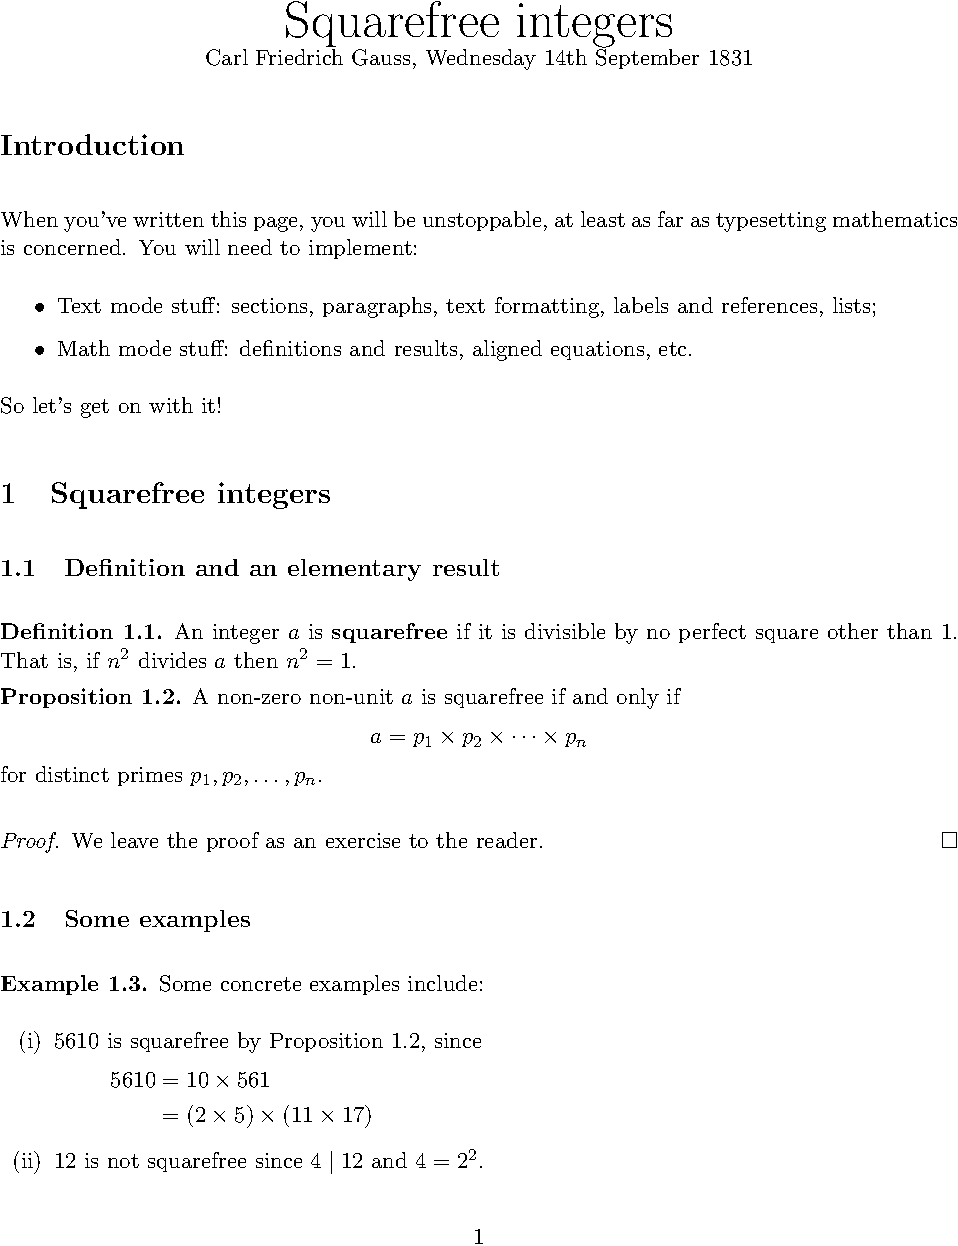
\includegraphics[keepaspectratio]{book/media/latex-exercise-crop.pdf}}}
\end{center}

\newpage
\subsection*{Template file}
\label{pTeXTemplate}

What follows is a template \texttt{.tex} file to get you started; it can be downloaded from \url{\bookurl/latex/}.

\lstinputlisting[basicstyle=\tt\scriptsize, xleftmargin=20pt, numbers=left]{book/media/template.tex}